% Evidence: M4-MICRO, RTX-MICRO, B570-FAST/SERIAL.
\begin{figure*}[t]
\centering
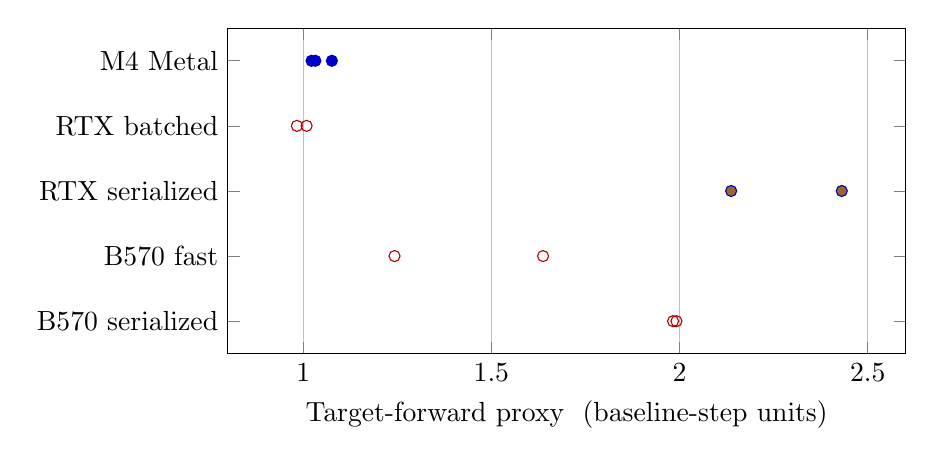
\begin{tikzpicture}
\begin{axis}[width=.84\textwidth,height=2.25in,xmin=.8,xmax=2.6,ymin=-.5,ymax=4.5,y dir=reverse,ytick={0,1,2,3,4},yticklabels={M4 Metal,RTX batched,RTX serialized,B570 fast,B570 serialized},xlabel={Target-forward proxy $\vTwo$ (baseline-step units)},xtick={1,1.5,2,2.5},xmajorgrids,axis on top]
\addplot[black,dashed,forget plot] coordinates {(1,-.5)(1,4.5)};
% Point pairs/triples at distinct contexts; not uncertainty intervals.
\addplot+[only marks,mark=*,color=blue!70!black] coordinates {(1.0221818546851145,0) (1.0761256101952625,0) (1.0322635228699184,0)};
\addplot+[only marks,mark=o,color=red!70!black] coordinates {(1.0090304299186035,1) (0.9831479829424705,1)};
\addplot+[only marks,mark=*,color=blue!70!black] coordinates {(2.43099575218514,2) (2.137011311768208,2)};
\addplot+[only marks,mark=o,color=red!70!black] coordinates {(1.2426,3) (1.6373,3)};
\addplot+[only marks,mark=o,color=red!70!black] coordinates {(1.982667717765499,4) (1.991706889255509,4)};

\end{axis}
\end{tikzpicture}
\caption{How does correctness change usable verification? Filled marks: paths exact on the frozen reported workloads; open marks: correctness-blocked paths (including B570 serialized). Each mark is one context cell; nearby cells can overlap. M4 contexts: 512/2048/8192; RTX 5070 Ti Laptop depths: 0/256; B570 contexts: 512/2048. Contexts, runtimes, and controls differ: this is not a hardware ranking. The plotted proxy is not complete $\rtarget$.}
\label{fig:verification}
\end{figure*}
